\section{Versuchsaufbau}
\label{sec:Versuchsaufbau}
\DeclareSIUnit{\liter}{l}
Für dieses Experiment werden ein Ultraschall Doppler-Generator im Pulsbetrieb, eine Ultraschallsonde mit einer Frequenz von $2\,\unit{\mega\hertz}$,
Strömungsrohre mit unterschiedlichen Innen- und Außendurchmessern und ein Computer für die Datenaufnahme und -analyse verwendet.. Bei diesem Versuch ist diese Flüssigkeit laminar, da sich der Messbereich in einer mittleren
Strömungsgeschwindigkeit befindet. Zusätzlich kann mithilfe einer Zentrifugalpumpe die Strömungsgeschwindigkeit von $0\,\sfrac{\unit{\liter}}{\unit{\minute}}$ bis $10\,\sfrac{\unit{\liter}}{\unit{\minute}}$
eingestellt werden. Allerdings soll für diesen Versuch eine Strömungsgeschwindigkeit von $7\,\sfrac{\unit{\liter}}{\unit{\minute}}$ nicht überschritten werden. 
\begin{wrapfigure}{r}{0.3\textwidth}
    \centering
    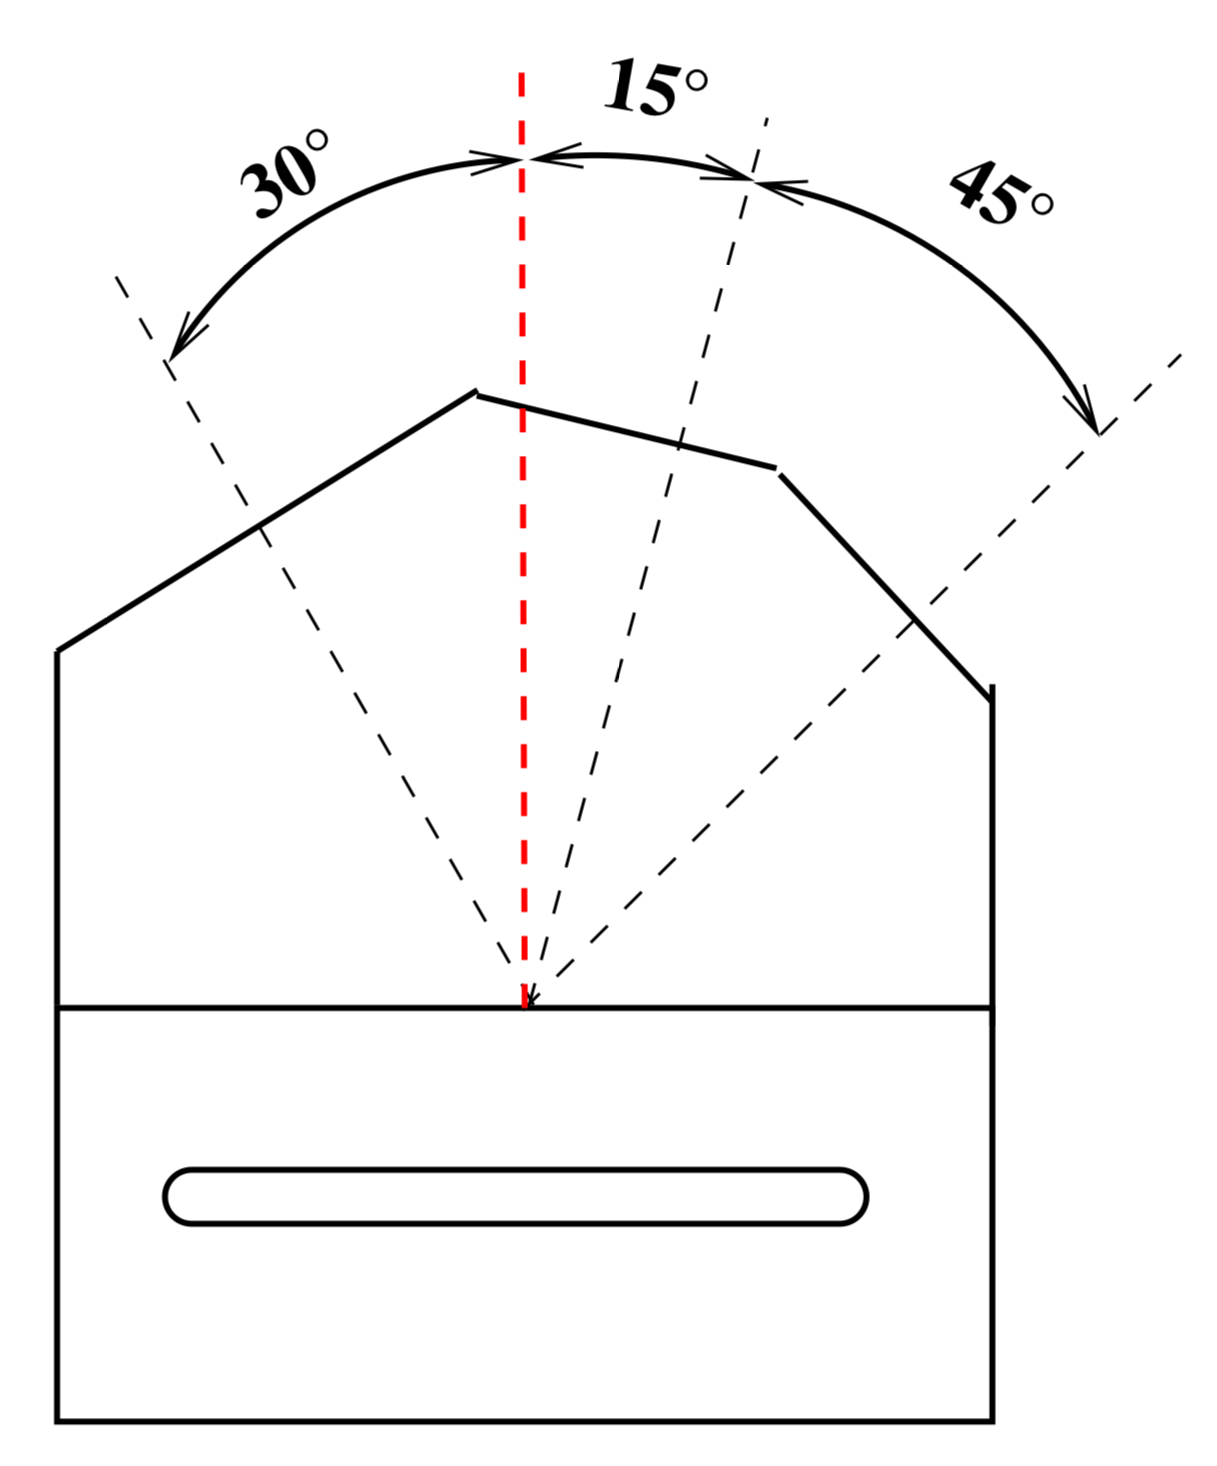
\includegraphics[width=0.29\textwidth]{content/Bilder/Prisma.jpeg}
    \caption{Skizze der verwendeten Doppler-Prismen Q\cite{anleitungUS3}.}
    \label{fig:Prisma}
\end{wrapfigure}
Auf dem Computer lassen sich die vom Echoskop gemessenen Daten 
mit der Messsoftware erfassen, anzeigen und auswerten.  Außerdem fließt eine Flüssigkeit (Dopplerphantomflüssigkeit), welche aus Wasser, Glycerin und Glaskugeln besteht, durch verschiedene
Des Weiteren wreden Doppler-Prismen mit drei verschiedenen Einschallwinkel, wie in Abbildung \ref{fig:Prisma} zu erkennen, verwendet. Diese werden für die Ankopplung der Ultraschallsonde genutzt und für jeden Rohrdurchmesser
ist ein Doppler-Prisma vorhanden. Der Abstand zwischen der Sonde und der Flüssigkeit ist für die drei verschiedenen Einstellwinkel gleich. Der Dopplerwinkel $\alpha$ wird über 
\begin{equation}
    \alpha = 90°-\arcsin\left( \sin \theta \cdot \frac{c_{\text{L}}}{c_{\text{P}}}\right)
    \label{eqn:Dopplerwinkel}
\end{equation}
berechnet. Hier beschreibt $c_{\text{L}}$ die Schallgeschwindigkeit der Dopplerflüssigkeit und $c_{\text{P}}$ die Schallgeschwindigkeit des Prismenmaterials und $\theta$ den Prismenwinkel.

\section{Durchführung}
\label{sec:Durchführung}
Als Erstes wird die Strömungsgeschwindigkeit als Funktion des Dopplerwinkels ermittelt. Hierfür
wird am Ultraschallgenerator bei den Geschwindigkeitsmessungen das SAMPLE VOLUME auf \textit{LARGE} eingestellt. Bei der Zentrifugalpumpe wird
\textbf{Mode M1} aktiviert. Dann wird mithilfe der Ultraschallsonde die Frequenzverschiebung $\Delta \nu$ für fünf verschiedene Flussgeschwindigkeiten gemessen.
Diese Messung wird an zwei Rohrdurchmessern mit allen drei Prismenwinkeln durchgeführt. 
Anschließend wird das Strömungsprofil der Doppler-Flüssigkeit bestimmt. Dabei wird die Frequenzverschiebung an zwei Rohren bei einem Prismenwinkel
von $15\,\unit{\degree}$ für verschiedene Messtiefen gemessen. Hier wird beim Ultraschallgenerator das SAMPLE VOLUME auf \textit{SMALL} eingestellt und die Messtiefen lassen sich bei dem DEPTH Regler
einstellen. Diese Messungen werden mit den Strömungsgeschwindigkeiten $3\,\sfrac{\unit{\liter}}{\unit{\minute}}$ und $6\,\sfrac{\unit{\liter}}{\unit{\minute}}$ durchgeführt.